\section{Ergebnisse}
\subsection{Anregungs- und Emissionspektrum von Pyren}
Ein Anregungs- und Emissionspektrum von Pyren in Ei-PC Vesikeln wurde für das Verhältnis 1:50 (Pyren:Ei-PC) bei der Temperatur $T=25^\circ C$ aufgenommen und in Abb. \ref{Em_Ex_Scan} dargestellt.
%Anregungs- und Emissionspektrum von Pyren
\begin{figure}[h!]
	\begin{center}
		\begin{minipage}{0,8\textwidth}
			
			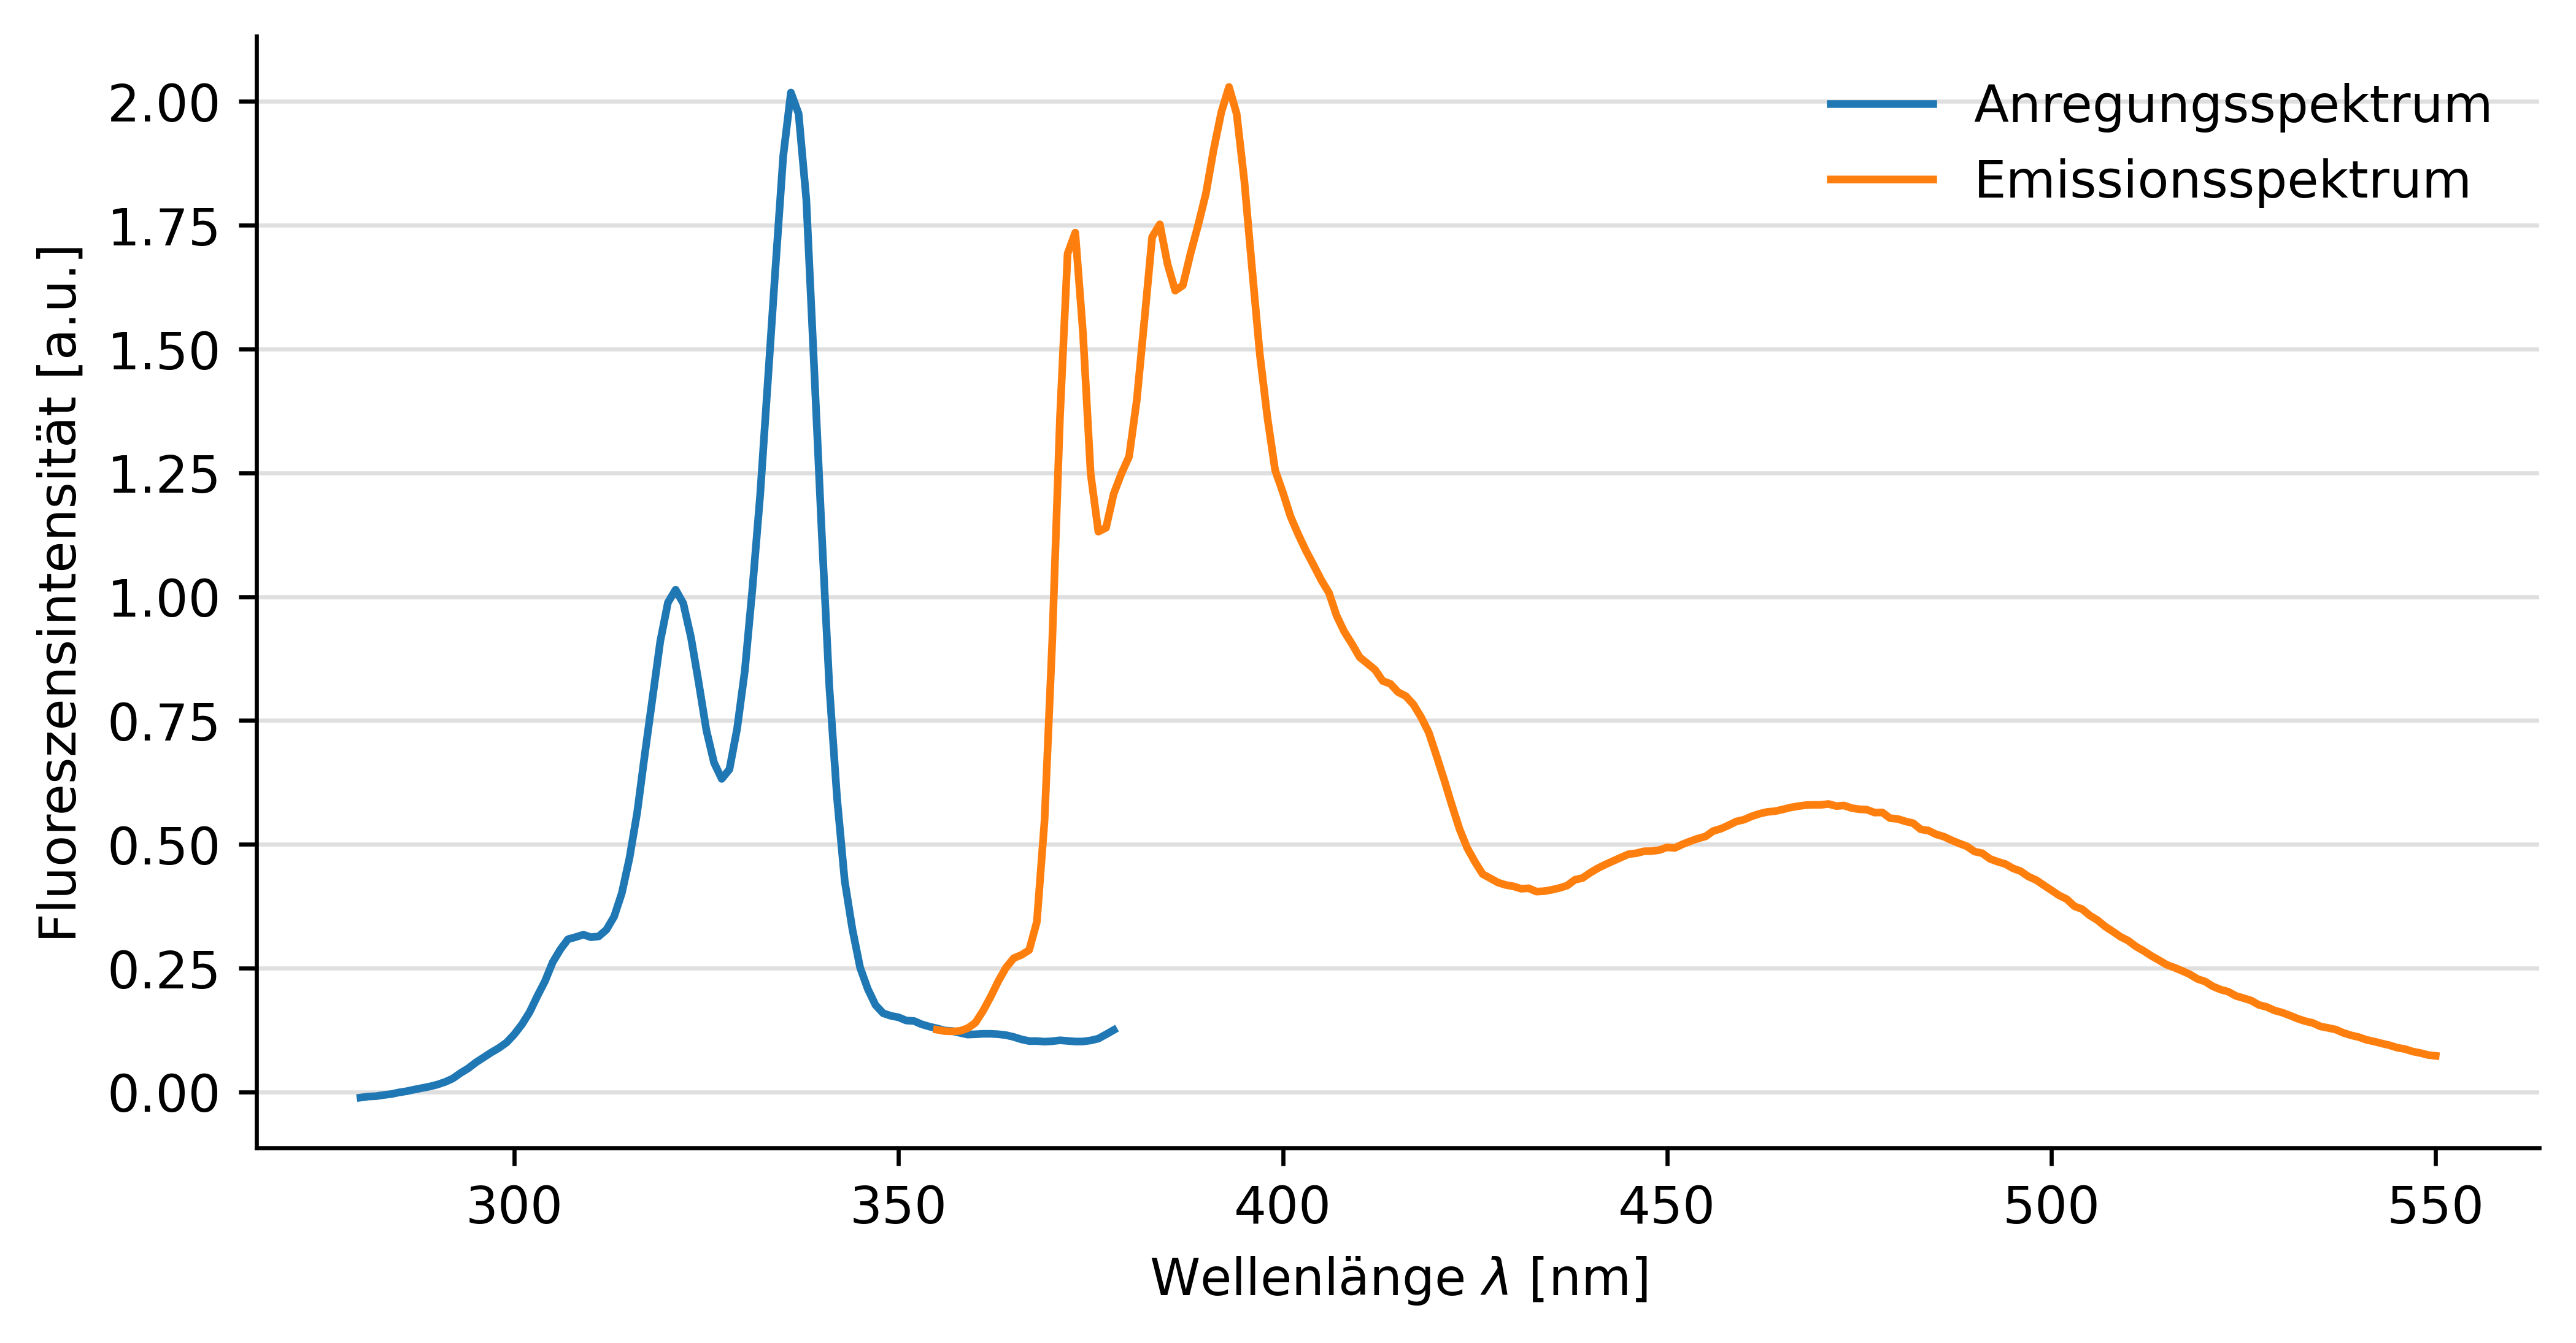
\includegraphics[width=\textwidth]{picture/Em_Ex_Scan_50.png}
			\caption{Anregungs- und Emissionspektrum von Pyren; Verhältnis 1:50 (Pyren:Ei-PC); $T=25^\circ C$, Versorgungsspanung Fluoreszenzspektrometer $U=550V$} 
			\label{Em_Ex_Scan} 
		\end{minipage}
	\end{center}
\end{figure}

\subsection{Fluoreszenzintensitäten des Monomers und des Excimers}
Im Folgenden wurde die Abhängigkeit der Fluoreszenzintensität der Monomere  ($\lambda=393$nm) und Excimere ($\lambda=470$nm) von der Pyrenkonzentration und von der Temperatur untersucht.\\
Am Gerät 3 wurden die Messungen von Pyren in Ei-PC und am Gerät 4 die Messungen von Pyren in DPPC aufgenommen.

\subsubsection{Fluoreszenzintensität als Funktion der Pyrenkonzentration}\label{sec:F_von_C}
In der Abb. \ref{Konz_Scan} sind die pyrenkonzentrationabhängingen Fluoreszenzintensität dargestellt. Die Messpunkte bei $\lambda=393$nm und bei $\lambda=470$nm wurden anschließend in Abb. \ref{Konz_Verh} zusammengetragen.

%ganzheitlicher Fluoreszenzintensität Scan 
\begin{figure}[h!]
	\begin{center}
		\begin{minipage}{0,8\textwidth}
			
			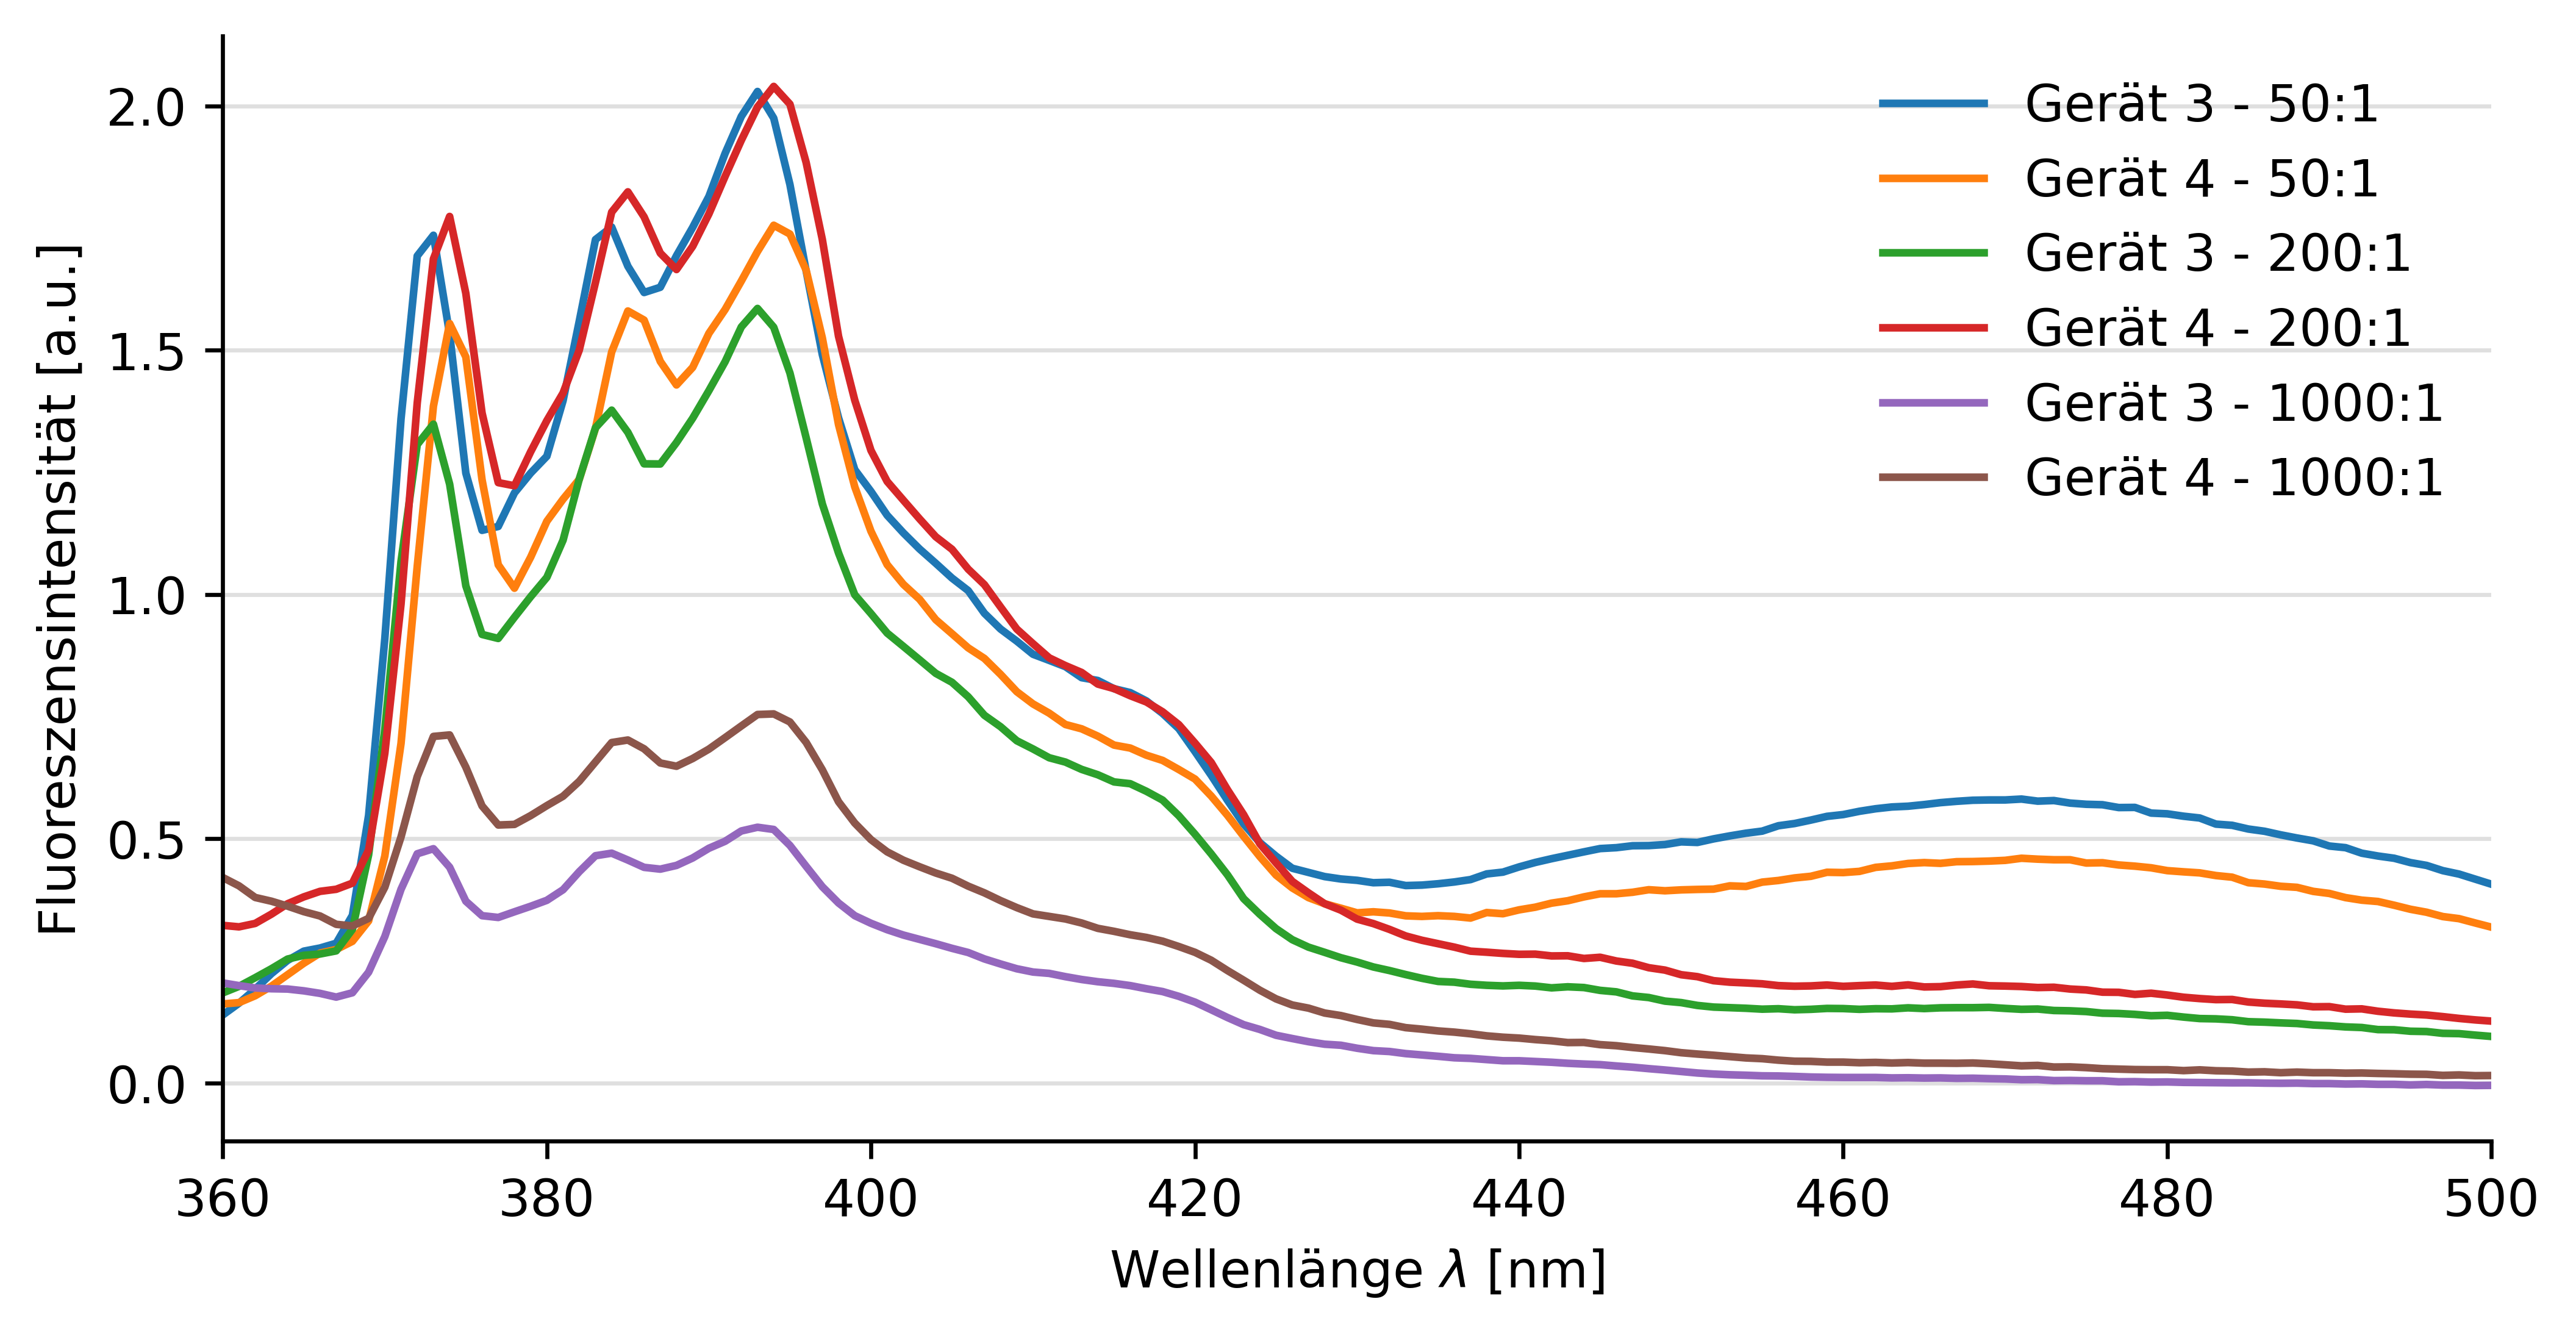
\includegraphics[width=\textwidth]{picture/Konz.png}
			\caption{Fluoreszenzintensität Spektrum von verschiedenen Ei-PC:Pyren-Verhältnissen} 
			\label{Konz_Scan} 
		\end{minipage}
	\end{center}
\end{figure}

%Fluoreszenzintensität als Funktion der Pyrenkonzentration
\begin{figure}[h!]
	\begin{center}
		\begin{minipage}{0,8\textwidth}
			
			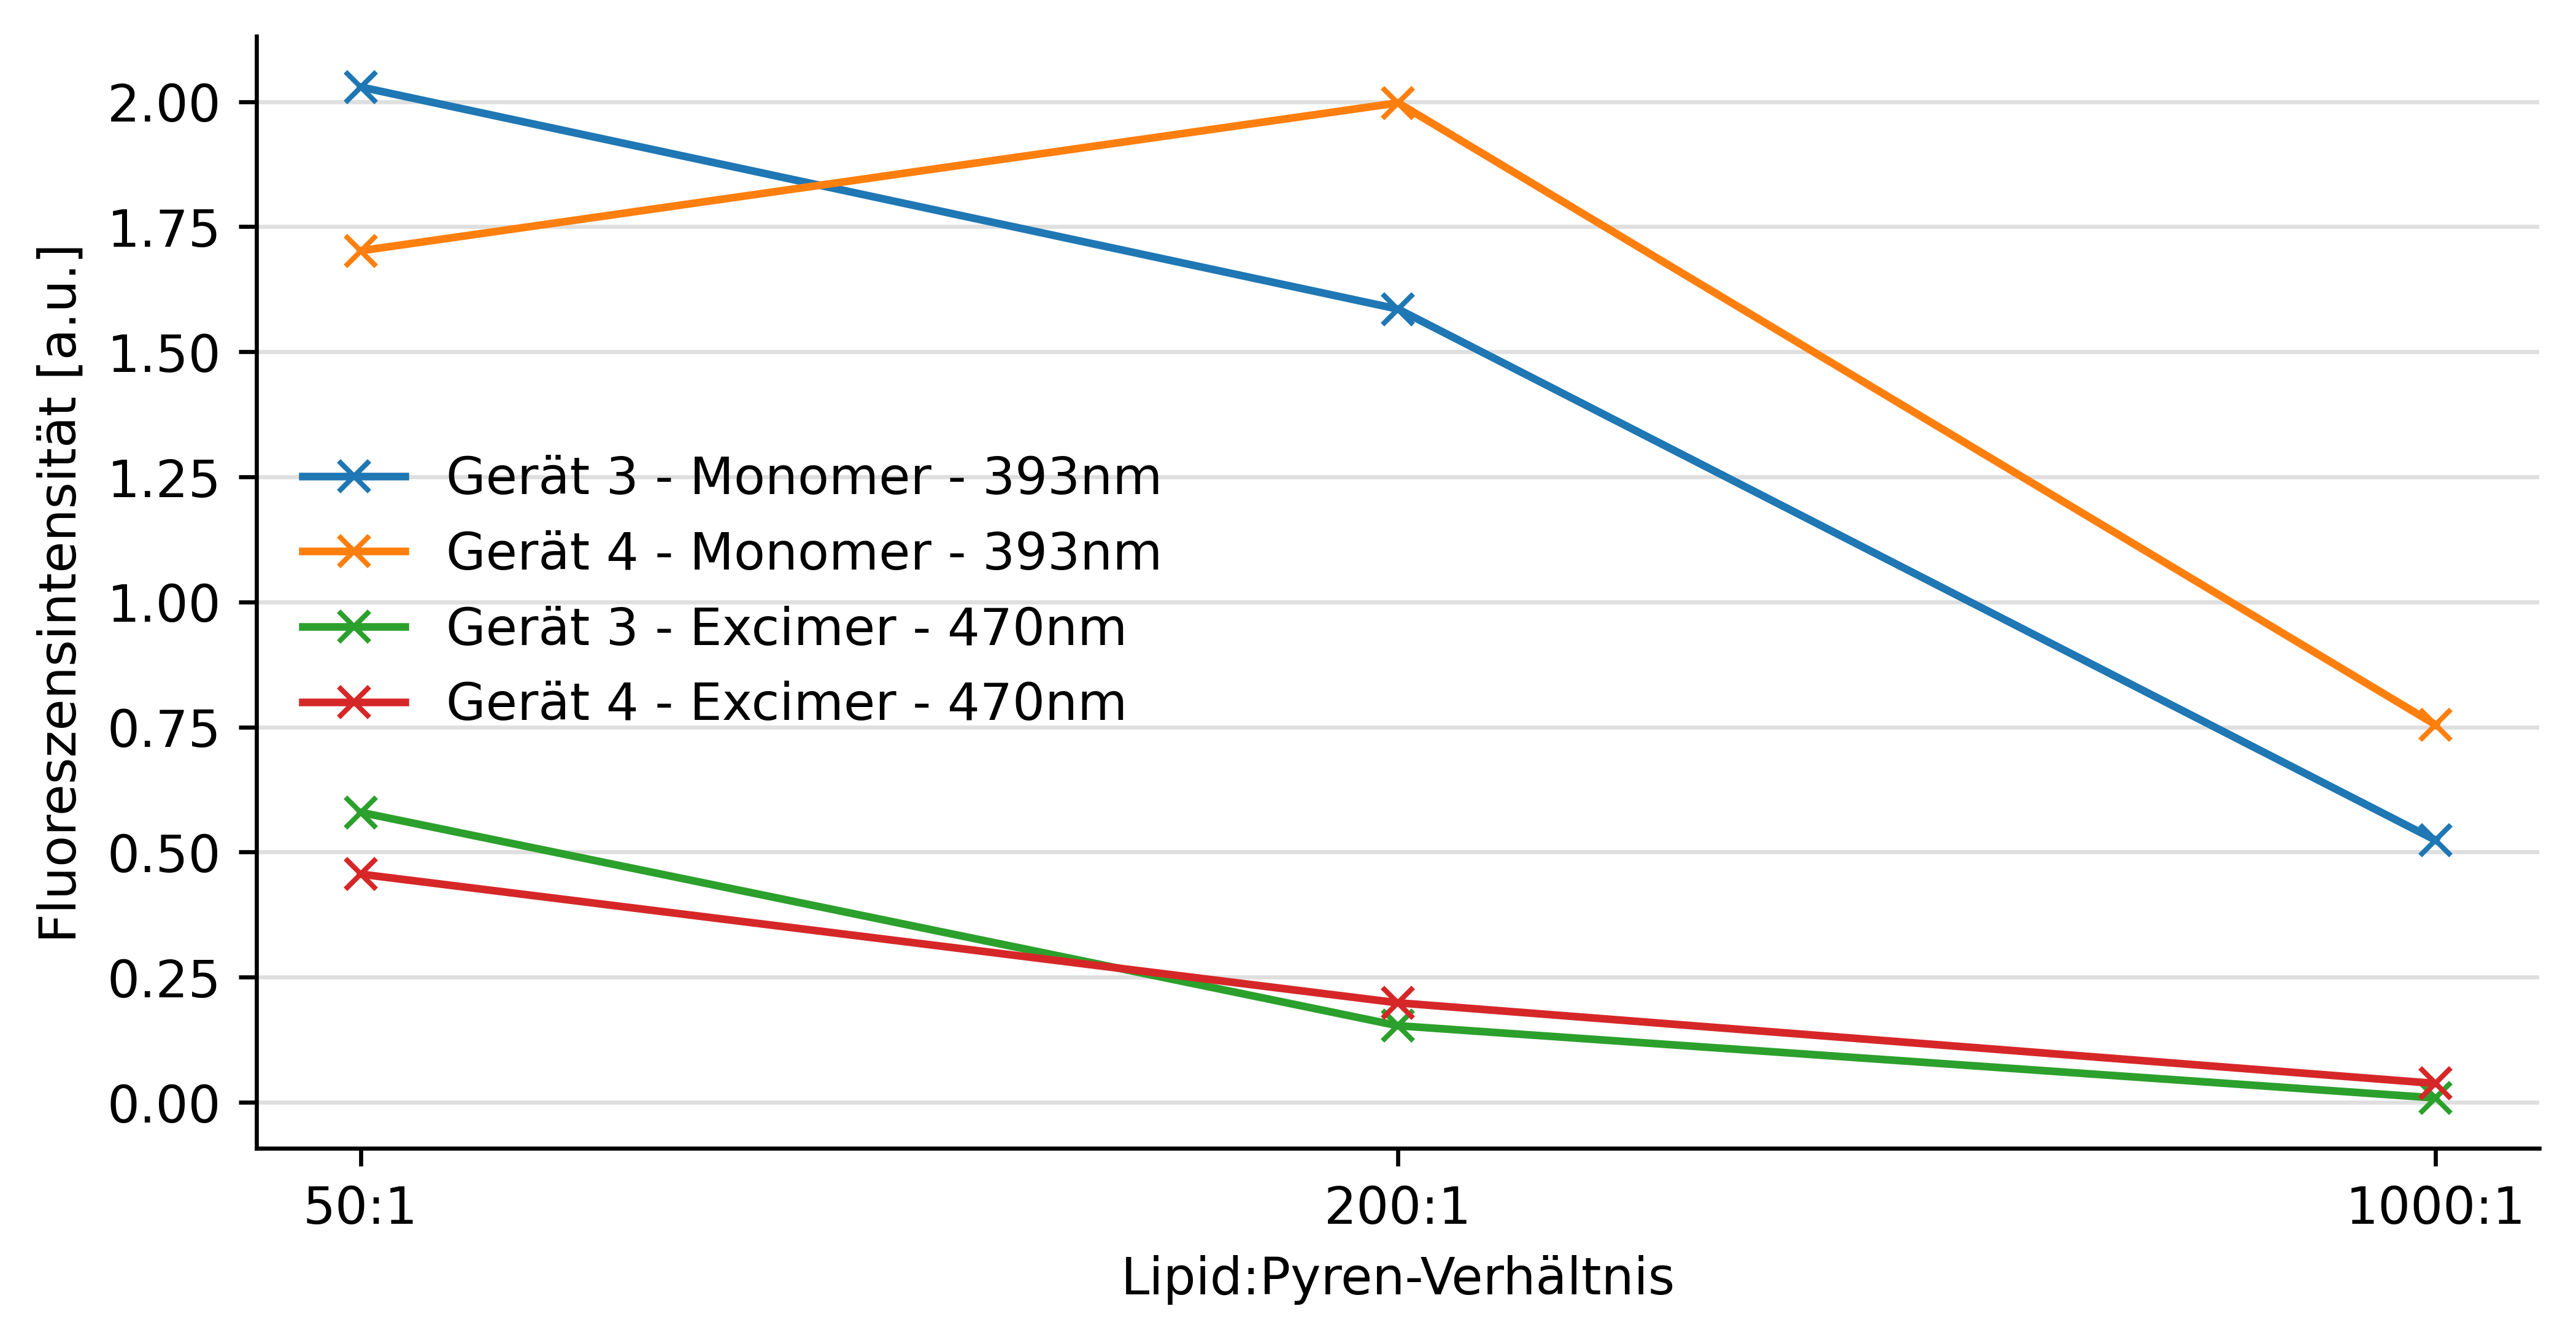
\includegraphics[width=\textwidth]{analysis/reports/Konz_Verh.png}
			\caption{Fluoreszenzintensität als Funktion des Ei-PC:Pyren-Verhältnis} 
			\label{Konz_Verh} 
		\end{minipage}
	\end{center}
\end{figure}
\vspace*{3.4cm}


\subsubsection{Fluoreszenzintensität als Funktion der Temperatur} \label{sec:FvonT}

Analog zum Verfahren aus dem Kapitel \ref{sec:F_von_C} wurden die Fluoreszenzmessdaten (bei Erhöhung der Temperatur im Messsystem) bestimmt und in den Abb. \ref{Monomer_Temp} und Abb. \ref{Excimer_Temp} dargestellt.

%Fluoreszenzintensität des Monomer als Funktion der Temperatur 
\begin{figure}[h!]
	\begin{center}
		\begin{minipage}{0,8\textwidth}
			
			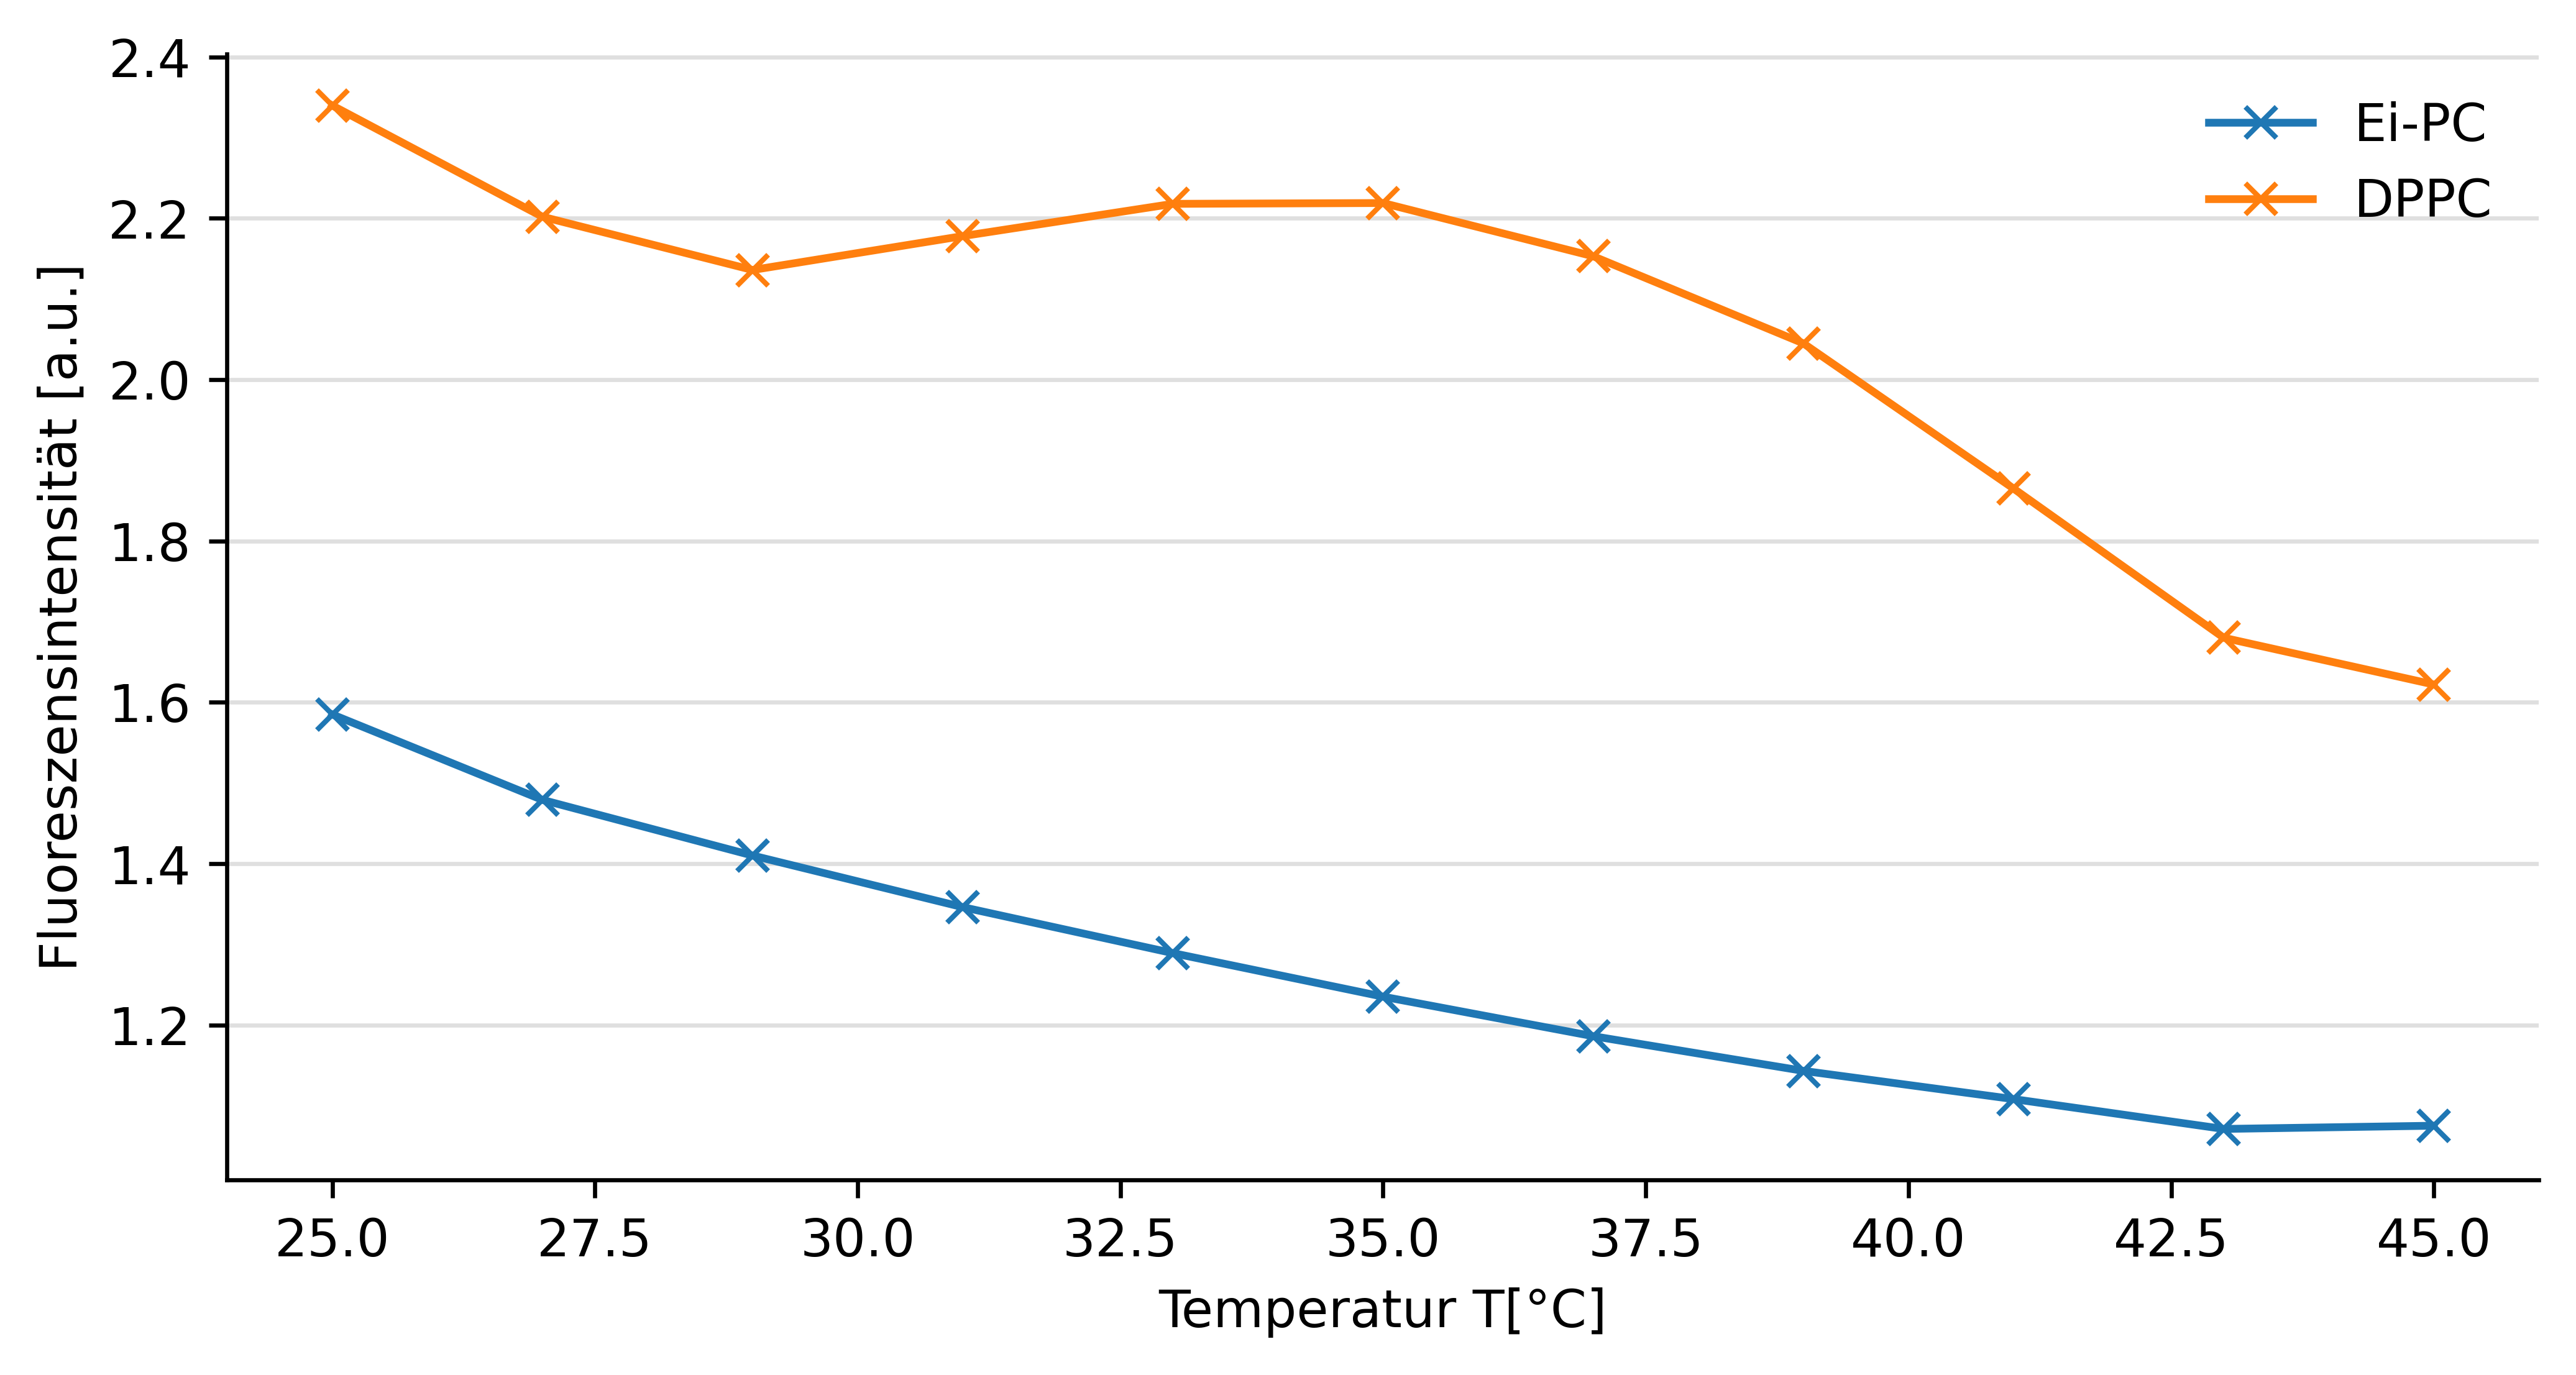
\includegraphics[width=\textwidth]{picture/Monomer_Temp.png}
			\caption{Pyren in Ei-PC bzw. DPPC Vesikeln; Fluoreszenzintensität des Monomer als Funktion der Temperatur} 
			\label{Monomer_Temp} 
		\end{minipage}
	\end{center}
\end{figure}

%Fluoreszenzintensität des Excimer als Funktion der Temperatur 
\begin{figure}[h!]
	\begin{center}
		\begin{minipage}{0,8\textwidth}
			
			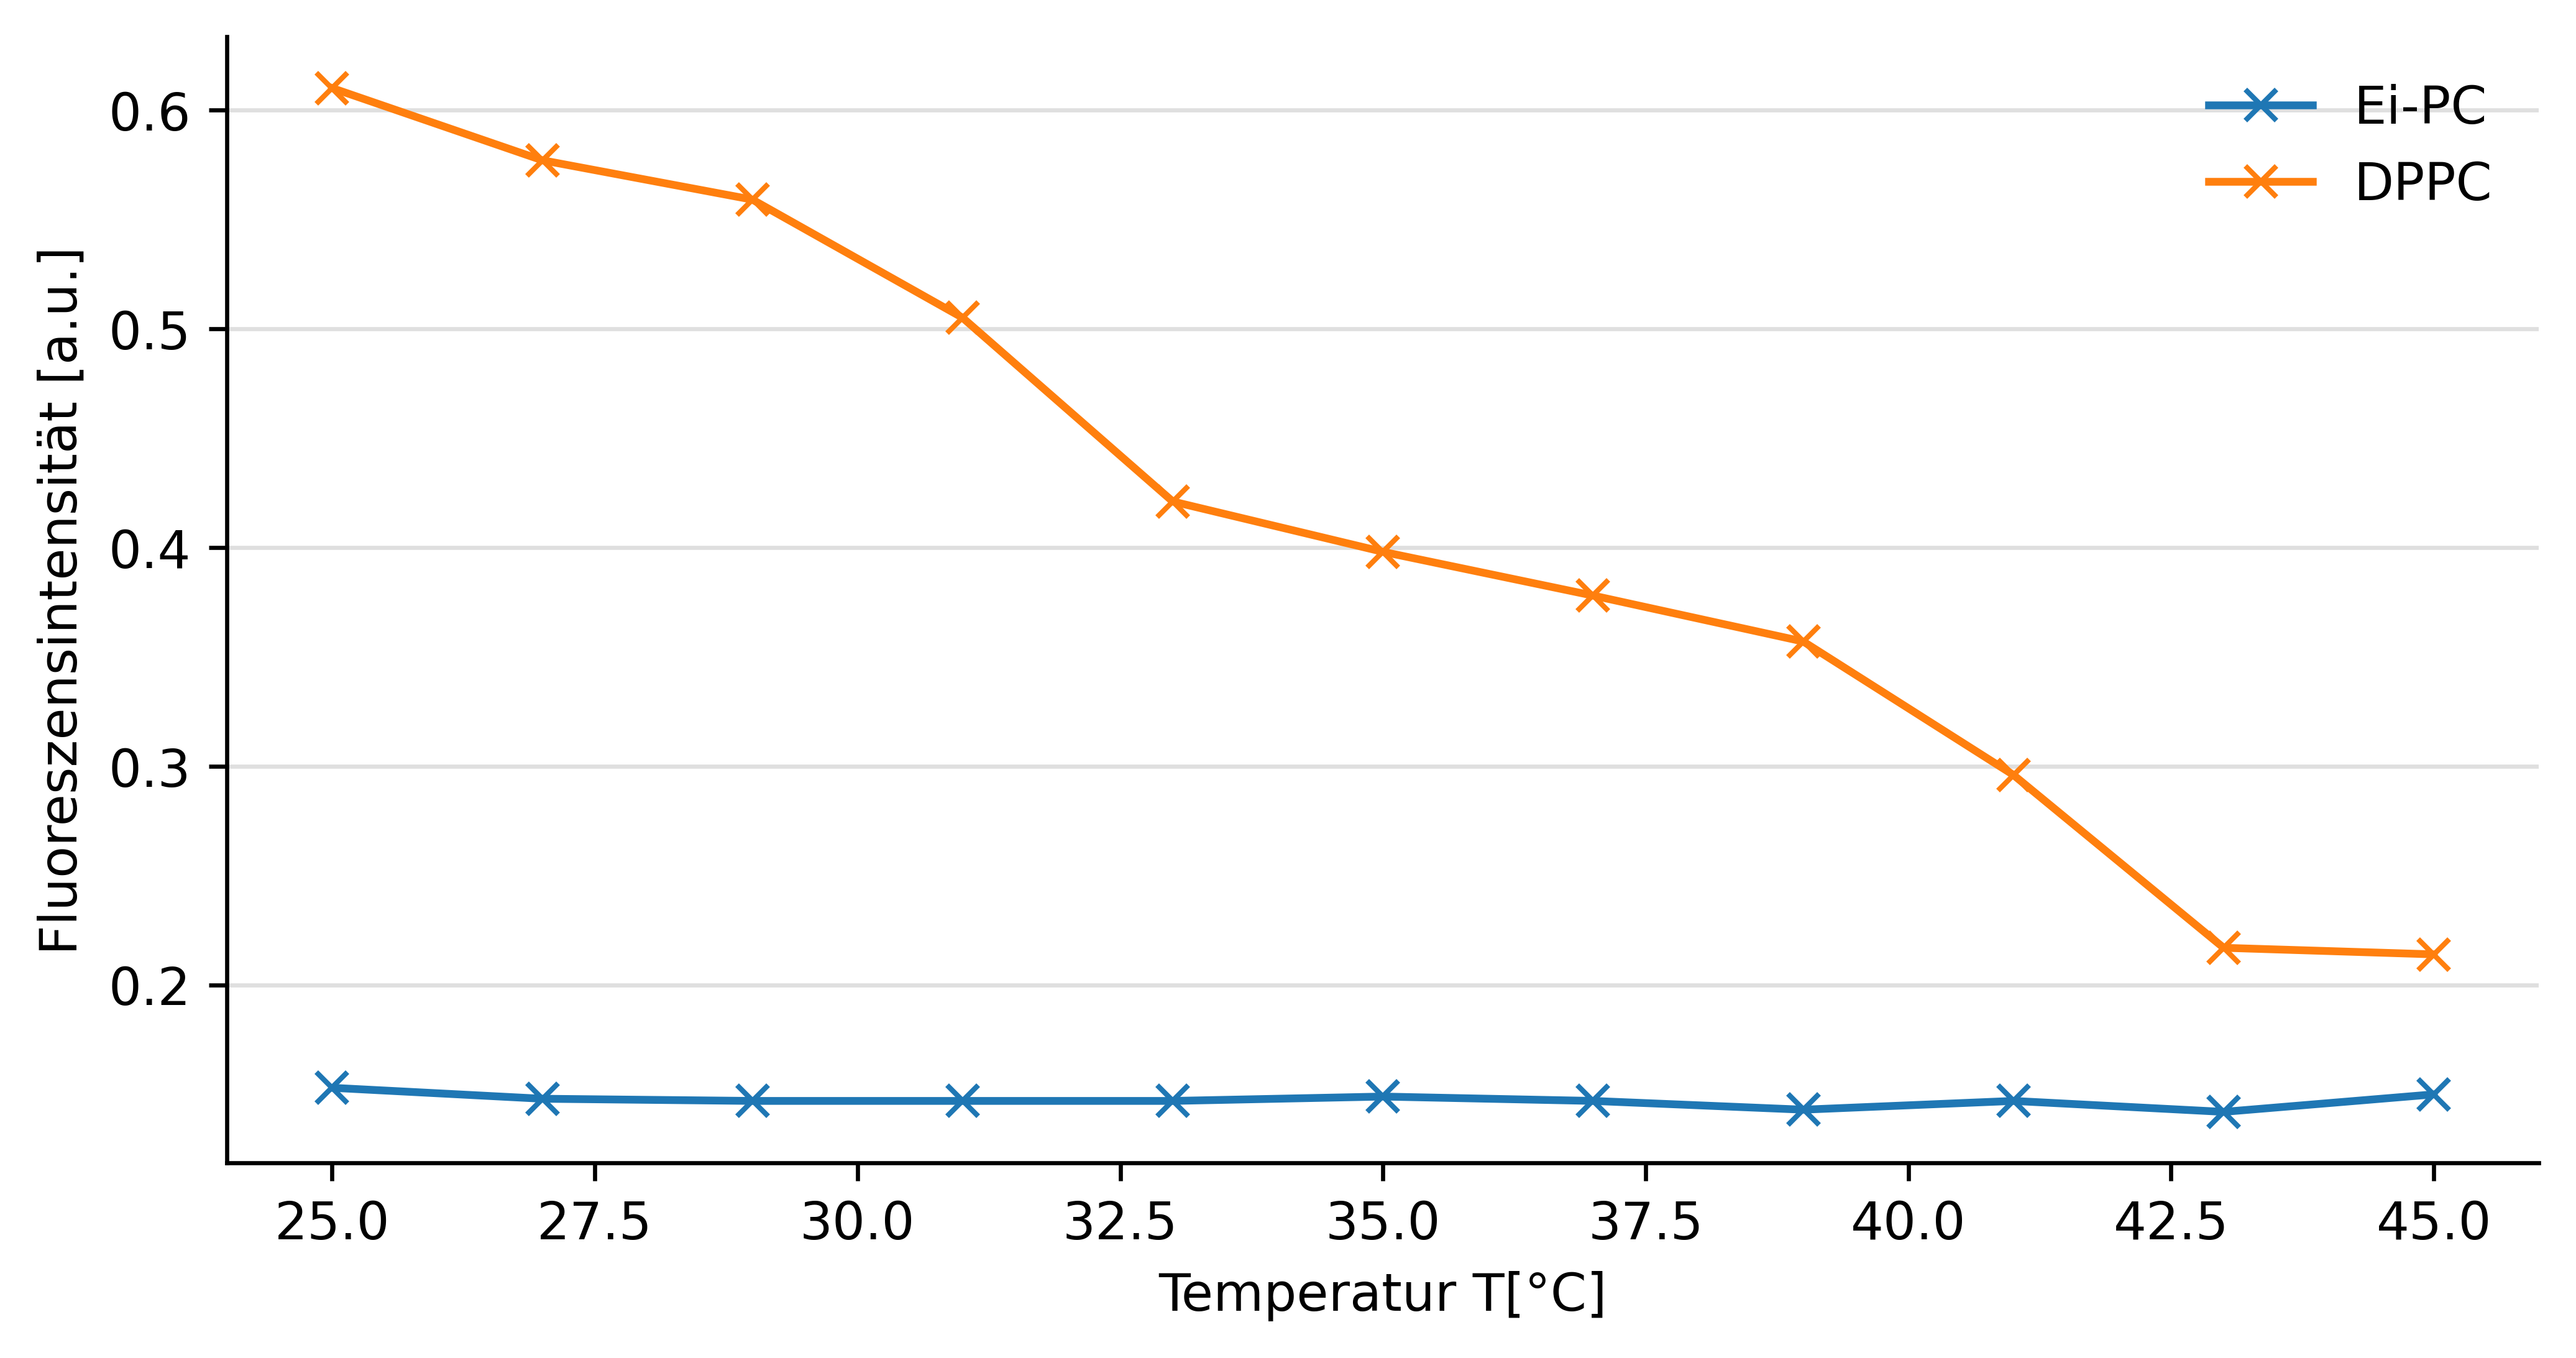
\includegraphics[width=\textwidth]{picture/Excimer_Temp.png}
			\caption{Pyren in Ei-PC bzw. DPPC Vesikeln; Fluoreszenzintensität des Excimer als Funktion der Temperatur} 
			\label{Excimer_Temp} 
		\end{minipage}
	\end{center}
\end{figure}

\subsection{Verhältnis Intensitäten Excimer:Monomer}\label{sec:Ex_Mono}
Folgend aus Kapitel \ref{sec:FvonT} wurde das Verhätlnis von Excimer (Abb. \ref{Excimer_Temp}) zu Monomer (Abb. \ref{Monomer_Temp}) berechnet und in Abb. \ref{Ex_Mono} geplottet.

%Verhältnis Intensitäten Excimer:Monomer für Pyren in Ei-PC bzw. DPPC
\begin{figure}[h!]
	\begin{center}
		\begin{minipage}{0,8\textwidth}
			
			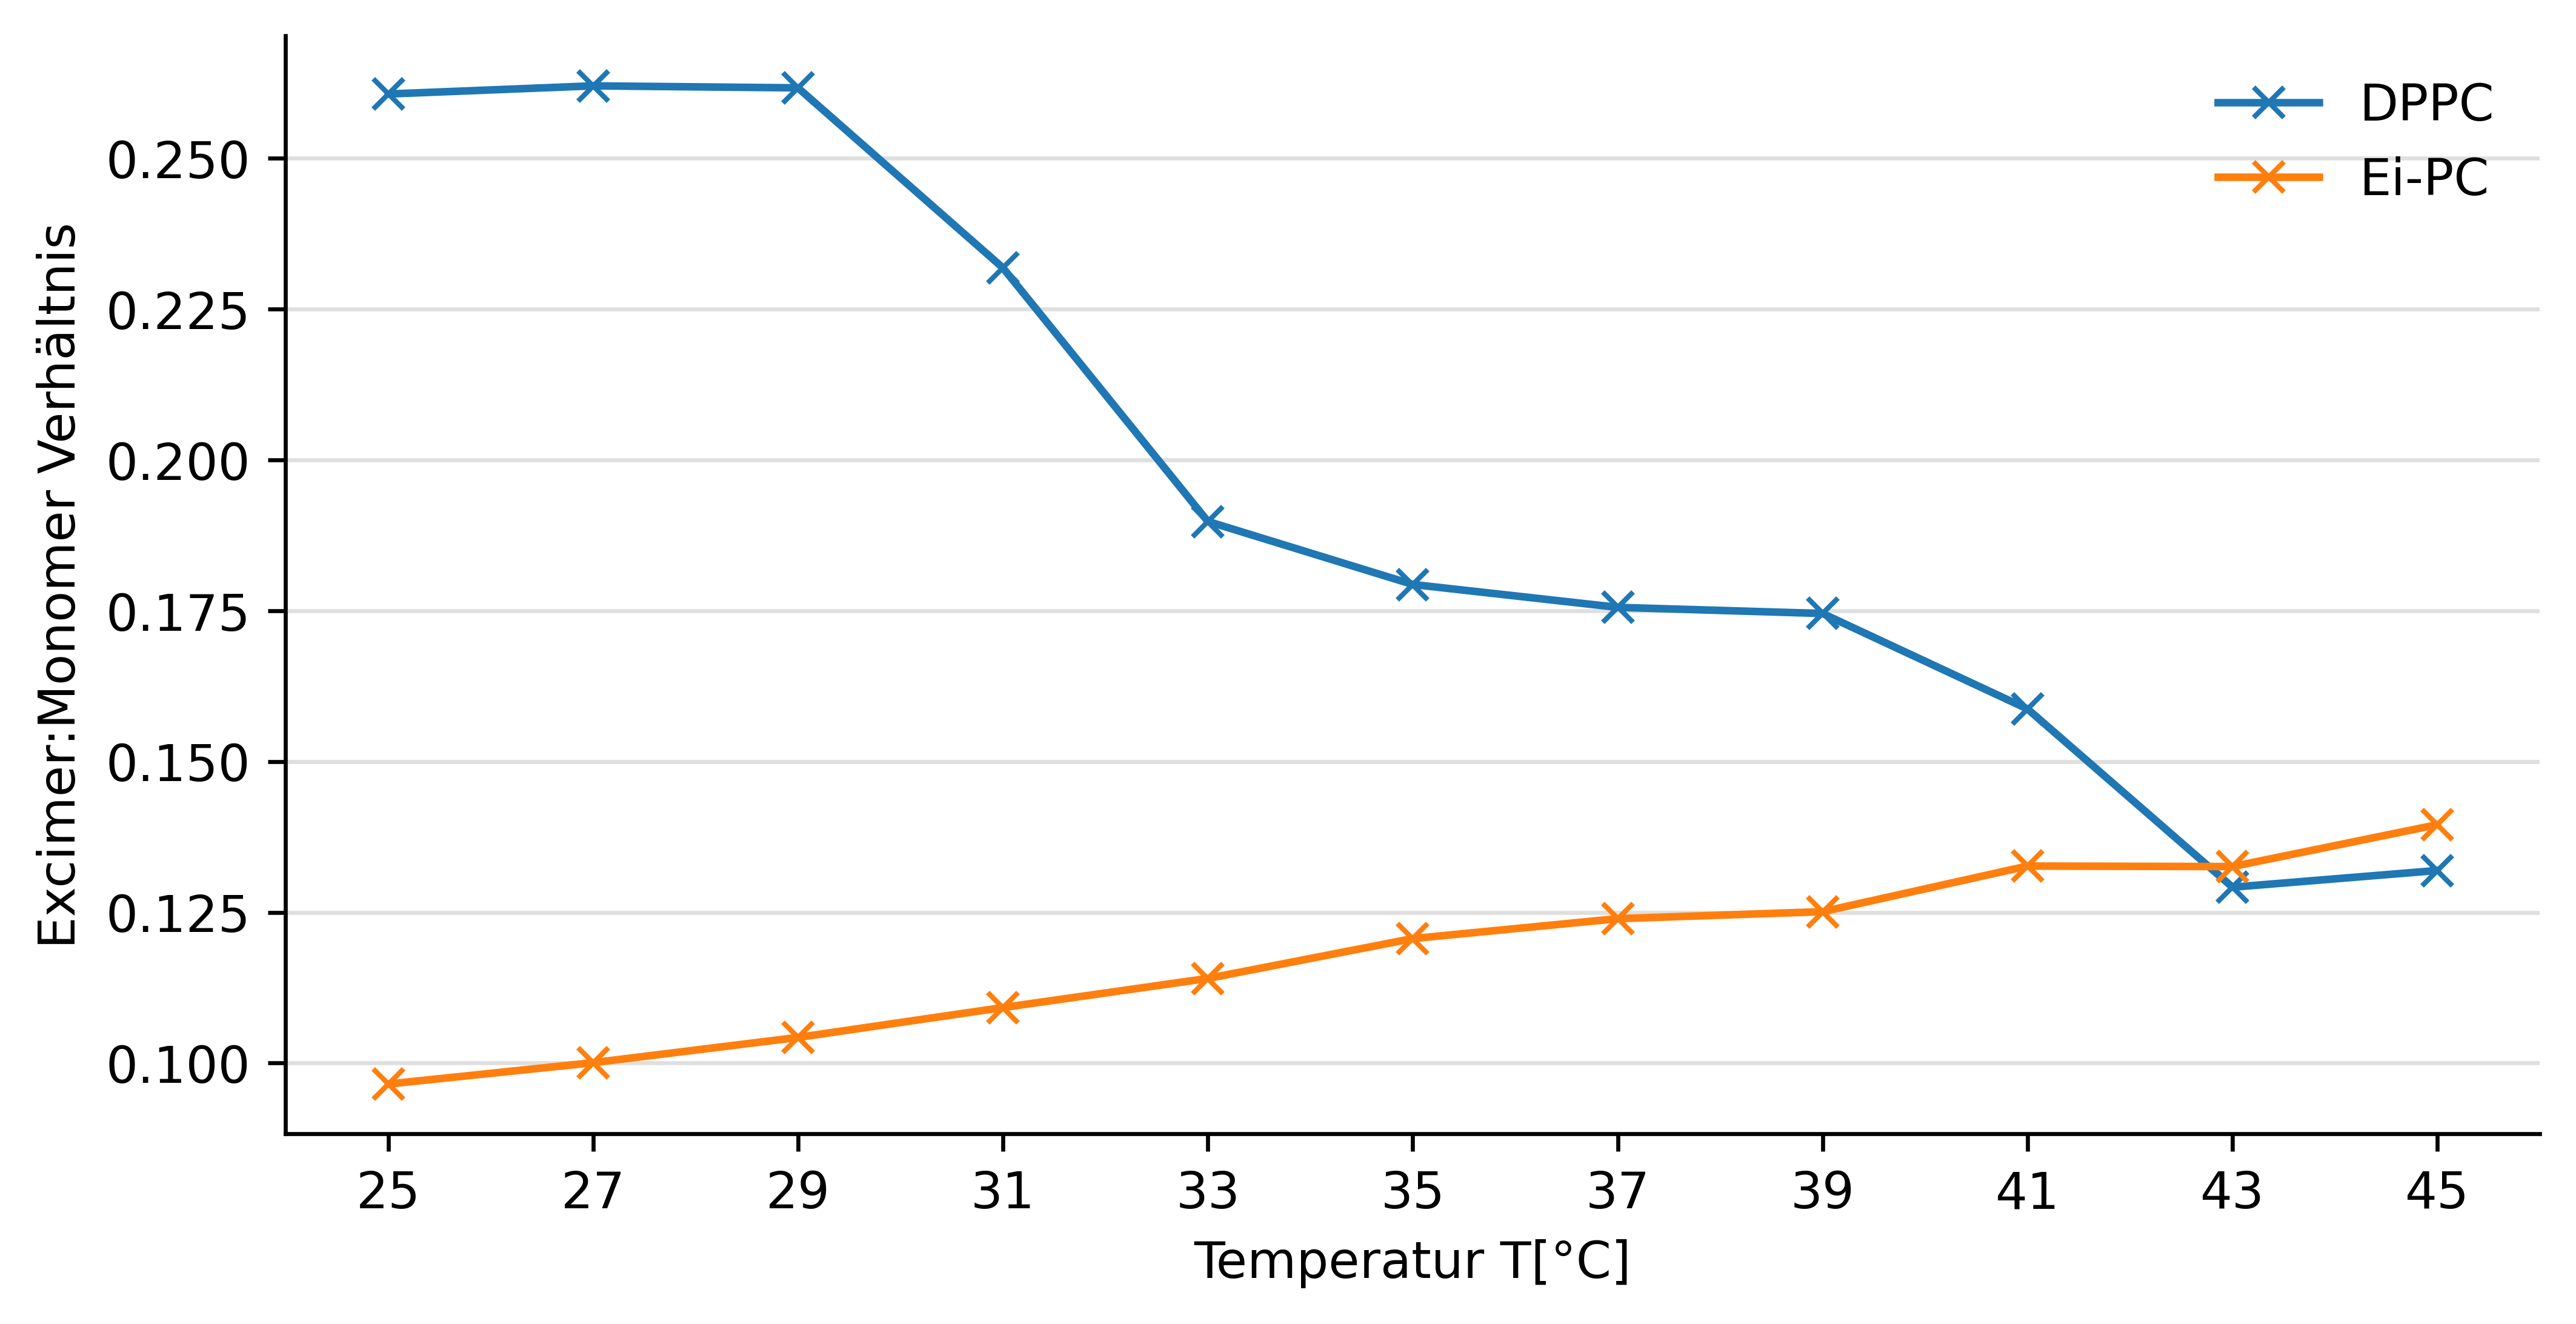
\includegraphics[width=\textwidth]{picture/Ex_Mono.png}
			\caption{Verhältnis Intensitäten Excimer:Monomer für Pyren in Ei-PC bzw. DPPC; Messung der Temperaturabhängigkeit} 
			\label{Ex_Mono} 
		\end{minipage}
	\end{center}
\end{figure}

\subsection{Lateraldiffusionskoeffizienten}
Die Berechnung der temperaturabhängigen Lateraldiffusionskoeffizienten $D_{diff}$ erfolgte analog zum Skript Seite 20 \cite{Kursskript} :\\
Aufbauend auf der Annahme einer $D_{diff}$ als Konzept einer Diffusion auf einem 2D Lipidgitter, wurde die Sprunghaftigkeit $\nu_i$ der Fluorophore von einem Gitterknotenpunkt zum Nächsten über die Formel \ref{formel1}
\begin{equation}\label{formel1}
\nu_i = <n_s> \frac{I'}{I\kappa}\frac{1}{\tau_0}\frac{k_f}{k_{f'}}
\end{equation}
mit der Formel \ref{formel2} 
\begin{equation}\label{formel2}
<n_s>=\frac{2}{\pi X_{py}}ln\frac{2}{X_{py}}
\end{equation}
zur Berücksichtigung der mittleren Sprungszahl zwischen zwei Kollisionen $<n_s>$  hinzugezogen.\\
$D_{diff}$ wurde anschließend über Formel \ref{formel3} berechnet.
\begin{equation}\label{formel3}
D_{diff}=\frac{1}{4}\nu_i \lambda^2
\end{equation}
Es gilt, dass die durchschnittliche Distanz im Lipidgitter $\lambda=0.8\text{nm}$, die Proportionalitätskonstante $\kappa=0.5$ und das Verhältnis der Fluoreszenzübergangsrate des Monomers bzw. Excimers $\frac{k_f}{k_{f'}}=0.1$ beträgt.\\\\
Formel \ref{formel1} und \ref{formel2} wurden anschließend mit den Parametern in die Formel \ref{formel3} eingesetzt und entsprechend gekürzt. \\
 Die temperaturabhängigen Fluoreszenzlebenszeiten des Excimers $\tau_0$
  \begin{table} [h]
 	\footnotesize
 	\begin{center}
 		\caption{Fluoreszenzlebenszeiten $\tau_0$ des Pyren-Excimers; temperaturabhängig}
 		\begin{tabular} {c c c l l l l l}
 			T[$^\circ$C]&  $\tau_0$ [ns] \\ \hline
 			25& 130 \\ \hline 
 			35&	115 \\ \hline 
 			45&	100 \\ \hline 
 		\end{tabular}
 		\label{tab:Lebenszeiten}
 	\end{center}
 \end{table}
wurden dem Skript entnommen.\\
Die Berechnung von $D_{diff}$ abhängig des molaren Anteils von Pyren $X_{py}$ und des in \ref{sec:Ex_Mono} berechneten Excimer:Monomer Verhältnissen (welche $\frac{I'}{I}$ entsprechen) erfolgte durch die gewonnene Formel \ref{formel4}

\begin{equation}\label{formel4}
D_{diff}=0.1\frac{1}{\pi X_{py}}ln\left(\frac{2}{X_{py}}\right)\frac{I'}{I}\frac{1}{\tau_0}\cdot0.64\text{nm}^2
\end{equation}
$X_{py}$ für die Messdaten zu Ei-PC und DPPC betrugen $X_{py}=5\cdot 10^{-3}$ 
%und für DPPC, da es bei annähernd gleicher Molaren Masse aber in 10-facher Menge vorhanden war, \\
%$X_{py,DPPC}=5\cdot 10^{-4}$. \\
Die jeweiligen Ergebnisse sind in der Tabelle \ref{tab:meinetabelle} dargestellt.

 \begin{table} [h]
	\footnotesize
	\begin{center}
		\caption{errechnete Diffusionskoeffizienten $D_{diff}$ von Pyren für ausgewählte Temperaturen}
		\begin{tabular} {c c c l l l l l}
			T[$^\circ$C]&  \multicolumn{2}{c}{$D_{diff}$ [$m^2s^{-1}$]} & \\ \hline
			&	Ei-PC&	DPPC \\ \hline 
			25&	1,81E-11&	1,15E-10\\ \hline 
			35&	2,56E-11&	8,45E-11\\ \hline 
			45&	3,41E-11&	5,23E-11\\ \hline 
		\end{tabular}
		\label{tab:meinetabelle}
	\end{center}
\end{table}


\newpage
